\documentclass[12pt]{article}

\usepackage{fancyhdr}  % Package for custom headers and footers
\usepackage{graphicx}  % Package to include images
\usepackage{array}     % Package for more flexible table columns
\usepackage{titlesec}  % Package for customizing section titles
\usepackage{geometry}  % Package for page margins

% Configure page margins
\geometry{
    top=1in,
    bottom=1in,
    left=1in,
    right=1in
}

% Set headheight to avoid warnings
\setlength{\headheight}{60pt}
\setlength{\topmargin}{-0.5in}
\setlength{\textheight}{9in}

% Configure the header for all pages
\pagestyle{fancy}
\fancyhf{}  % Clear all header and footer fields
\fancyhead[L]{
\includegraphics[height=1.5cm]{recursos_img/tec_header_logo.png}}  % Insert image in the left header
\fancyhead[R]{\parbox[b]{7cm}{\raggedleft \textbf{Comité institucional de ética en la investigación.\\ Propuesta de protocolo de investigación.}}}

\begin{document}

% Title with header
\begin{flushleft}
    \textbf{\Large Implementación de una Interfaz Cerebro-Computadora basada en P300 para el Control e Interacción de Robots}
    \par
    \textbf{15 de Agosto de 2024}
\end{flushleft}

\section{Investigador principal}

\begin{table}[h!]
    \centering
    \begin{tabular}{|c|p{7cm}|} \hline
        Nombre & Javier Mauricio Antelis Ortíz \\ \hline
        Cargo & Profesor - Investigador \\ \hline
        Institución de adscripción & Tecnológico de Monterrey \\ \hline
        División a la cual pertenece & Departamento de Computación \newline Escuela de Ingeniería y Ciencias \\ \hline
        Dirección electrónica & mauricio.antelis@itesm.mx \\ \hline
        Grado máximo de estudio & Doctorado \\ \hline
        Disciplina & Ingeniería Biomédica y Computación \\ \hline
        Especialidad & Neurotecnología e Interfaces Cerebro-Computador \\ \hline
    \end{tabular}
\end{table}

\begin{table}[h!]
    \centering
    \begin{tabular}{|c|p{7cm}|} \hline
        Nombre & Omar Mendoza Montoya \\ \hline
        Cargo & Profesor - Investigador \\ \hline
        Institución de adscripción & Tecnológico de Monterrey \\ \hline
        División a la cual pertenece & Departamento de Computación \newline Escuela de Ingeniería y Ciencias \\ \hline
        Dirección electrónica & omendoza83@tec.mx \\ \hline
        Grado máximo de estudio & Doctorado \\ \hline
        Disciplina & Ingeniería Biomédica y Computación \\ \hline
        Especialidad & Neurotecnología e Interfaces Cerebro-Computador \\ \hline
    \end{tabular}
\end{table}

\section{Investigadores asociados}

\begin{table}[h!]
    \centering
    \begin{tabular}{|c|c|} \hline
        Eleazar Olivas Gaspar & A01731405@tec.mx \\ \hline
        Janet Meza Hernández & A01747907@tec.mx \\ \hline
        Allan Hernández López & A01351947@tec.mx \\ \hline
        Manuel Alejandro Ramos Valdez & A00227837@tec.mx \\ \hline
        José Oswaldo Sobrevilla Vázquez & A01412742@tec.mx \\ \hline
        Hector Silverio Ceron Soto & A01638843@tec.mx \\ \hline
    \end{tabular}
\end{table}

\section{Duración del protocolo}

\begin{table}[h!]
    \centering
    \begin{tabular}{|c|c|} \hline
        Inicio & 5 de Agosto de 2024 \\ \hline
        Fin & 26 de Noviembre de 2024 \\ \hline
    \end{tabular}
\end{table}

\section{Tipo de experimentación}
Experimental y aplicativa.

\section{Línea de investigación}
Neurociencias, Tecnologías de la Computación, Robótica.

\section{Lugar de la investigación}
Laboratorio de Neurotecnología e Interfaces Cerebro-Computador (NTLab), Edificio
 del Ecosistema de Ingeniería, Arquitectura y Diseño (EIAD), 
 Tecnológico de Monterrey, Guadalajara.

\section{Resumen}

\subsection{Introducción y Justificación}
La electroencefalografía (EEG) es una técnica no invasiva ampliamente 
utilizada para registrar la actividad eléctrica del cerebro. 
Esta tecnología ha permitido avances significativos en la creación 
de interfaces cerebro-computadora (BCI), que utilizan señales cerebrales para 
controlar dispositivos externos. Uno de los enfoques emergentes es la integración 
de BCI con otras tecnologías, como sistemas de seguimiento ocular (eye tracking), 
para crear interfaces híbridas que ofrecen nuevas posibilidades en la interacción 
humano-robot.

\subsection{Objetivo de la Investigación}
Este protocolo de investigación tiene como objetivo desarrollar y evaluar dos 
tipos de interfaces híbridas para el control de brazos robóticos (Dobots) en un 
entorno de competencia. En el primer experimento, se combinará un sistema de eye 
tracking con la detección de potenciales relacionados a errores (ErrP) obtenidos 
por EEG para controlar un brazo robótico en tareas de escritura y dibujo. 
En el segundo experimento, se compararán los tiempos de respuesta y la eficiencia 
entre una BCI basada en P300 y un sistema de eye tracking en la tarea de controlar 
dos Dobots jugando tic-tac-toe. Un brazo robótico será controlado por la BCI, 
mientras que el otro será gestionado mediante el eye tracker.

\subsection{Metodología}
Los participantes, todos mayores de edad, serán seleccionados para utilizar 
estas tecnologías en el control de los Dobots. Se registrarán tanto las señales 
EEG como los datos de seguimiento ocular durante las tareas. El desempeño de los 
sistemas se evaluará en términos de precisión, tiempo de respuesta y eficiencia en 
la ejecución de las tareas asignadas.

\subsection{Impacto y Aplicaciones Futuras}
Los resultados de este estudio proporcionarán una visión clara sobre la viabilidad 
y eficacia de las interfaces híbridas en el control de dispositivos robóticos. 
Este conocimiento es crucial para el desarrollo de soluciones tecnológicas que 
pueden restaurar la autonomía de individuos con discapacidades motoras, abriendo 
nuevas posibilidades para aplicaciones en rehabilitación y asistencia robótica. 
Además, este proyecto sentará las bases para futuras investigaciones y desarrollos 
en el campo de las interfaces cerebro-computadora y su integración con tecnologías 
de seguimiento ocular.

\section{Objetivo}
El objetivo principal de este estudio es desarrollar y evaluar la eficacia de 
interfaces híbridas para el control de brazos robóticos utilizando tecnologías de 
seguimiento ocular y electroencefalografía (EEG). Específicamente, el estudio se 
centrará en los siguientes objetivos:

\begin{itemize}
    \item \textbf{Desarrollar un sistema híbrido de control}: Integrar un sistema de eye tracking con la detección de potenciales relacionados a errores (ErrP) obtenidos a partir de señales EEG para controlar un brazo robótico en tareas de escritura y dibujo.
    \item \textbf{Comparar la eficacia de las interfaces}: Evaluar y comparar el rendimiento de una interfaz cerebro-computadora (BCI) basada en el paradigma P300 frente a un sistema de eye tracking en la tarea de controlar dos brazos robóticos en un juego de tic-tac-toe.
    \item \textbf{Medir la precisión y eficiencia}: Analizar la precisión, tiempo de respuesta y eficiencia de los sistemas de control en la ejecución de las tareas asignadas, con el fin de determinar cuál de las tecnologías ofrece un control más rápido y eficiente de los brazos robóticos.
    \item \textbf{Explorar aplicaciones futuras}: Identificar posibles aplicaciones y mejoras de las interfaces híbridas en el contexto de rehabilitación robótica y asistencia tecnológica, así como su potencial impacto en la restauración de la autonomía en individuos con discapacidades motoras.
\end{itemize}

Estos objetivos buscan proporcionar una comprensión detallada de la viabilidad y 
las ventajas de integrar tecnologías de seguimiento ocular y EEG para el control 
de dispositivos robóticos, lo cual podría representar un avance significativo en 
la interacción humano-robot y en el desarrollo de soluciones tecnológicas para la 
asistencia en la vida diaria.

\section{Hipótesis}
En el presente estudio, se propone la integración de una interfaz 
cerebro-computadora (BCI) para el control de dos brazos robóticos. Se evaluará si 
el uso de un BCI basado en el paradigma P300 puede proporcionar un control más 
rápido y eficiente en comparación con el seguimiento ocular a través de eye 
trackers. Dado que ambos métodos permiten la interacción con los brazos robóticos, 
se espera que el BCI basado en P300 ofrezca un tiempo de respuesta inferior, 
debido a su capacidad de captar directamente las señales neuronales relacionadas 
con la intención de movimiento, en contraposición al seguimiento ocular, que 
depende de movimientos físicos y tiempo de procesamiento adicional.

\section{Participantes}

\subsection{Tamaño de la muestra}
Para el protocolo de investigación se reclutarán 30 adultos que cumplan con los 
criterios de inclusión.

\subsection{Criterios de inclusión}
\begin{itemize}
    \item Ser mayor de edad.
    \item Género y sexo indistintos.
    \item Mantener funciones cognitivas relacionadas con la atención, orientación, y memoria.
    \item No presentar trastornos musculoesqueléticos que impidan el movimiento normal.
    \item Consentimiento informado para participar en el estudio.
\end{itemize}

\subsection{Criterios de exclusión}
\begin{itemize}
    \item Diagnóstico de enfermedades neurodegenerativas.
    \item Diagnóstico de alteraciones severas en la atención.
    \item Antecedentes de traumatismo craneoencefálico.
    \item Lesiones de nervio periférico, enfermedad vascular cerebral.
    \item Contracturas que limiten la movilidad.
    \item Condiciones que puedan introducir datos con alto nivel de ruido.
\end{itemize}

\section{Material y equipo}
El equipo necesario para la investigación incluye:
\begin{itemize}
    \item Dispositivos de EEG para la captura de señales cerebrales.
    \item Sistemas de seguimiento ocular (eye trackers) para registrar movimientos oculares.
    \item Dos brazos robóticos Dobots para las tareas experimentales.
    \item Computadoras con software de análisis de datos y control de robots.
    \item Espacio adecuado para la instalación de los equipos y realización de los experimentos.
\end{itemize}

\begin{figure}[h!]
    \centering
    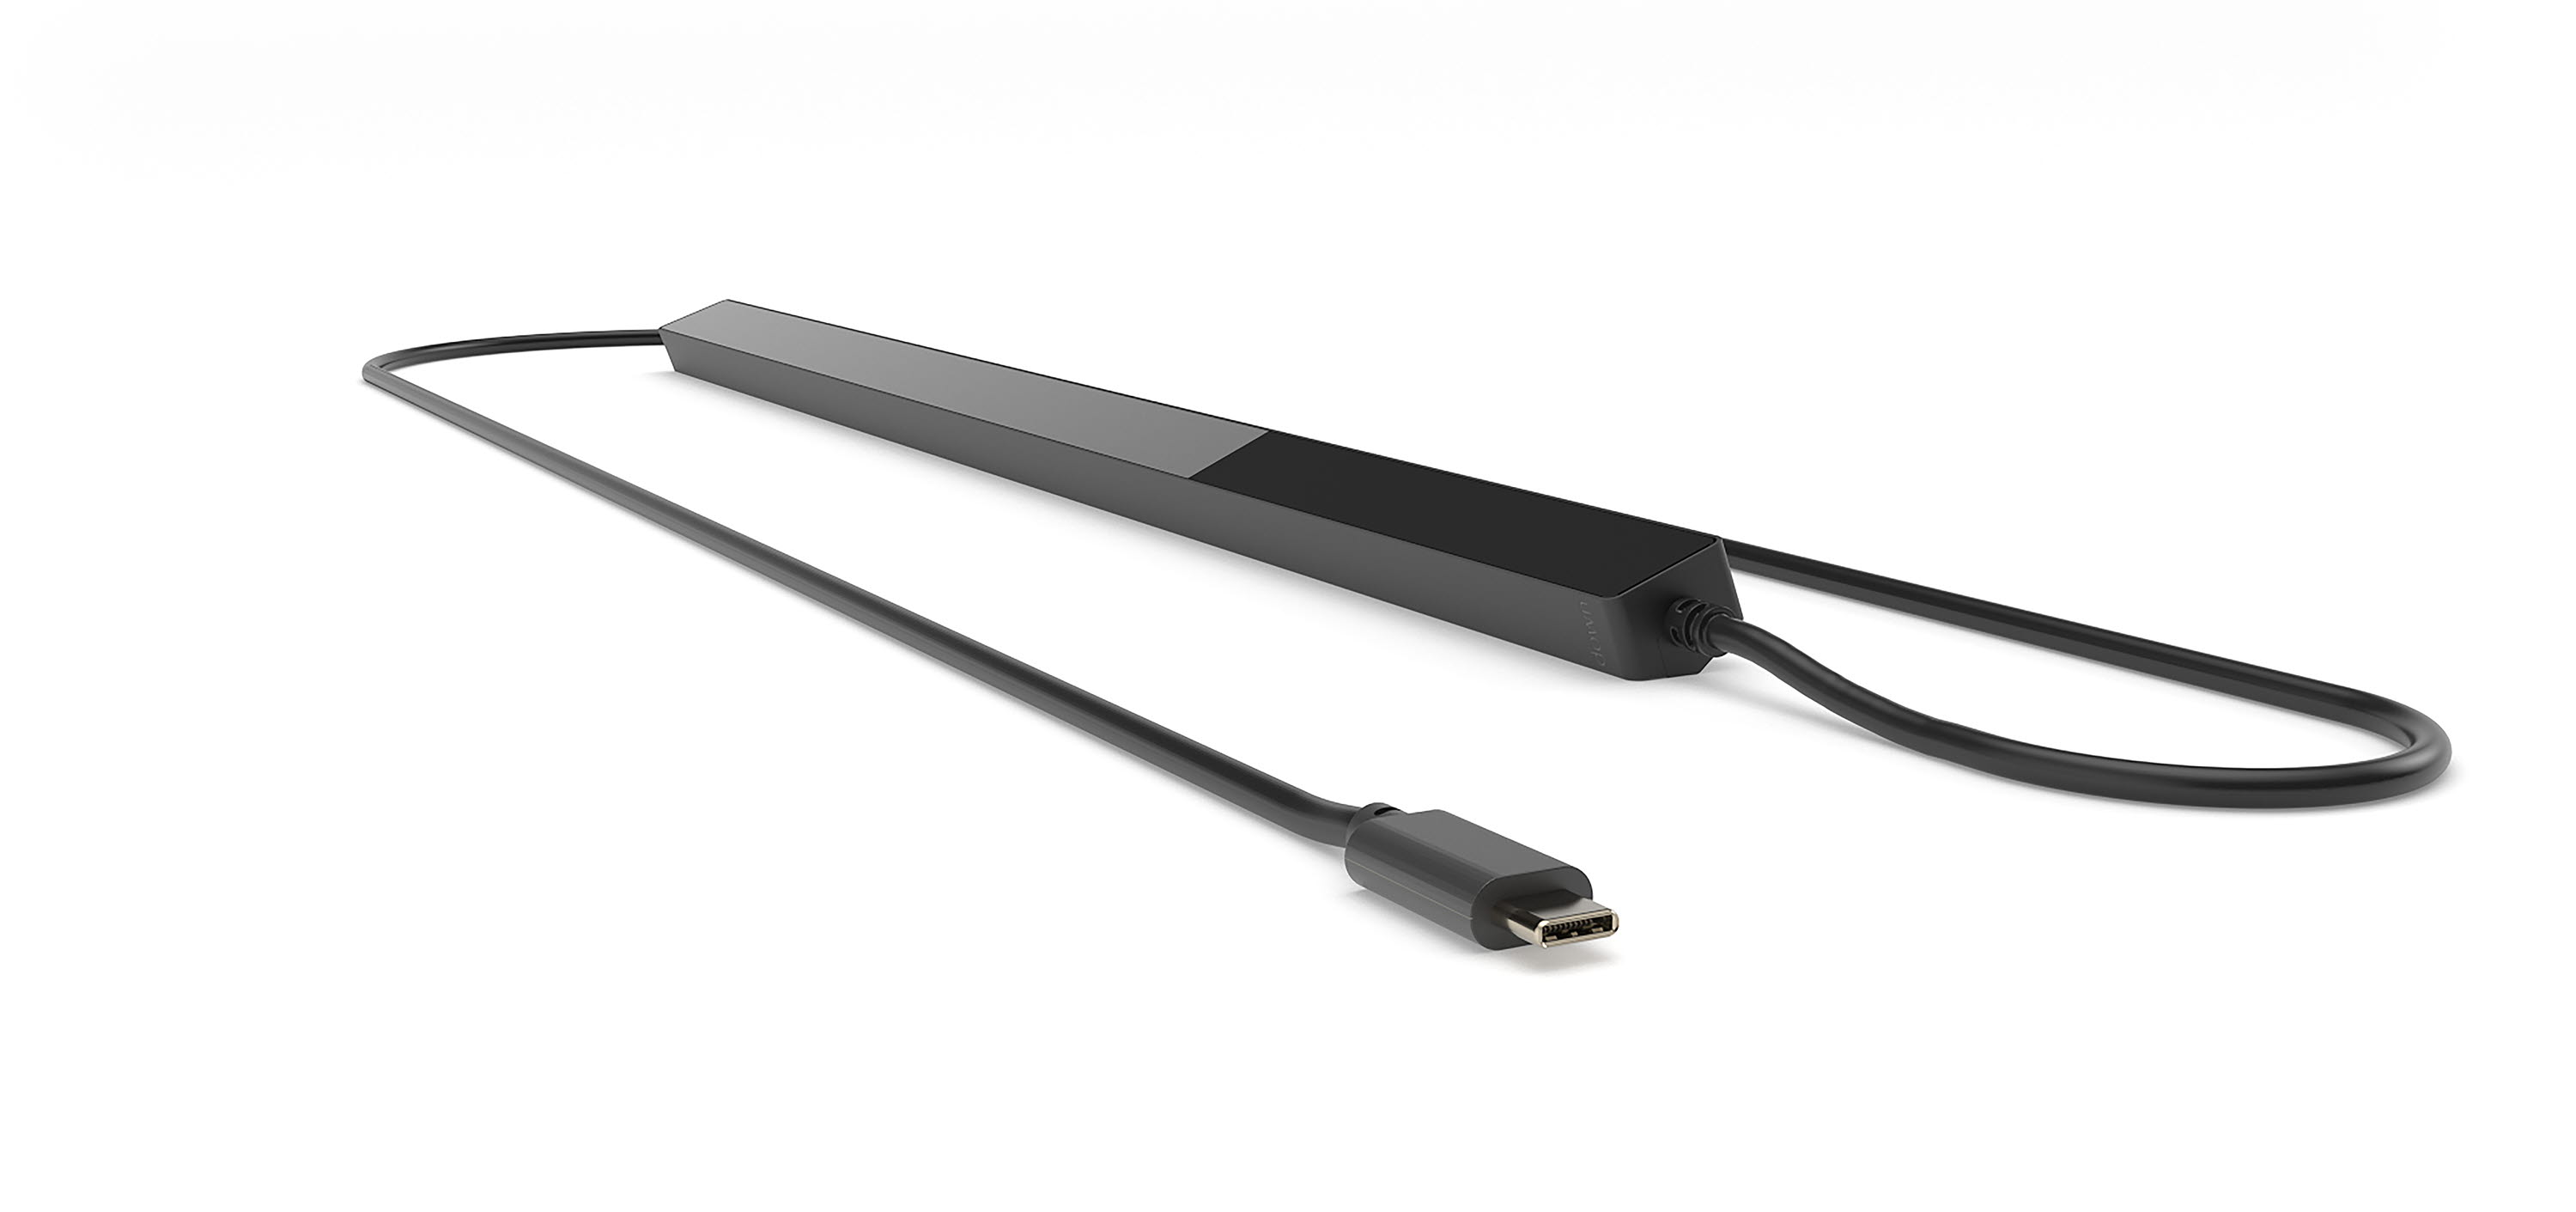
\includegraphics[width=0.4\textwidth]{recursos_img/tobii_fusion_pro.jpg}  % Ajusta la ruta y el ancho según sea necesario
    \caption{Tobii fusion pro eye tracker.}
    \label{fig:mi_imagen}  % Etiqueta para referencias cruzadas en el documento
\end{figure}

\begin{figure}[h!]
    \centering
    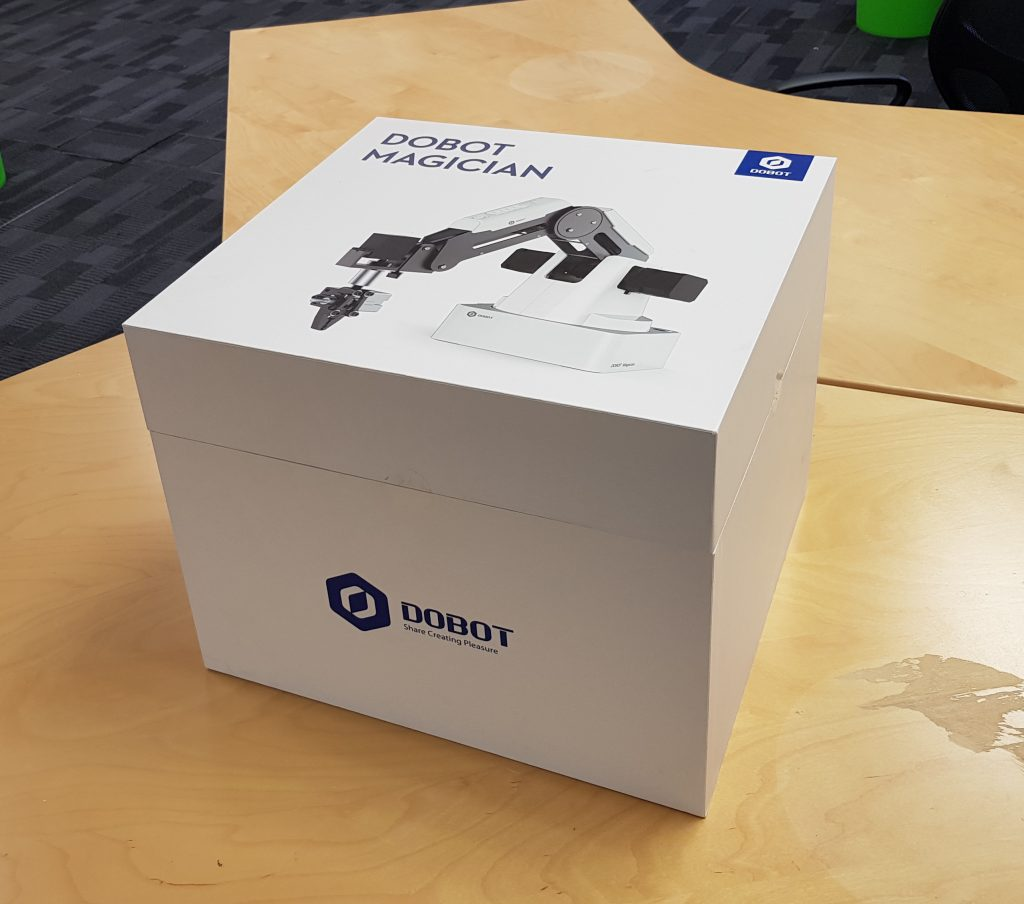
\includegraphics[width=0.4\textwidth]{recursos_img/dobot_magician.jpg}  % Ajusta la ruta y el ancho según sea necesario
    \caption{Brazo robotico Dobot magician.}
    \label{fig:mi_imagen}  % Etiqueta para referencias cruzadas en el documento
\end{figure}

\section{Descripción del procedimiento experimental}
Durante el experimento, los participantes serán instruidos sobre el uso de los 
sistemas de eye tracking y BCI. Se realizarán pruebas en las que deberán controlar 
los brazos robóticos para realizar tareas específicas, como escribir, dibujar o 
jugar tic-tac-toe. Se registrarán las señales EEG y los datos de seguimiento 
ocular, y se evaluará la precisión, tiempo de respuesta y eficiencia de ambos 
métodos.

\subsection{Preparación del equipo}
Previo a la realización del experimento se deberá hacer la preparación 
adecuada del equipo que se estará usando durante el mismo.

\begin{figure}[h!]
    \centering
    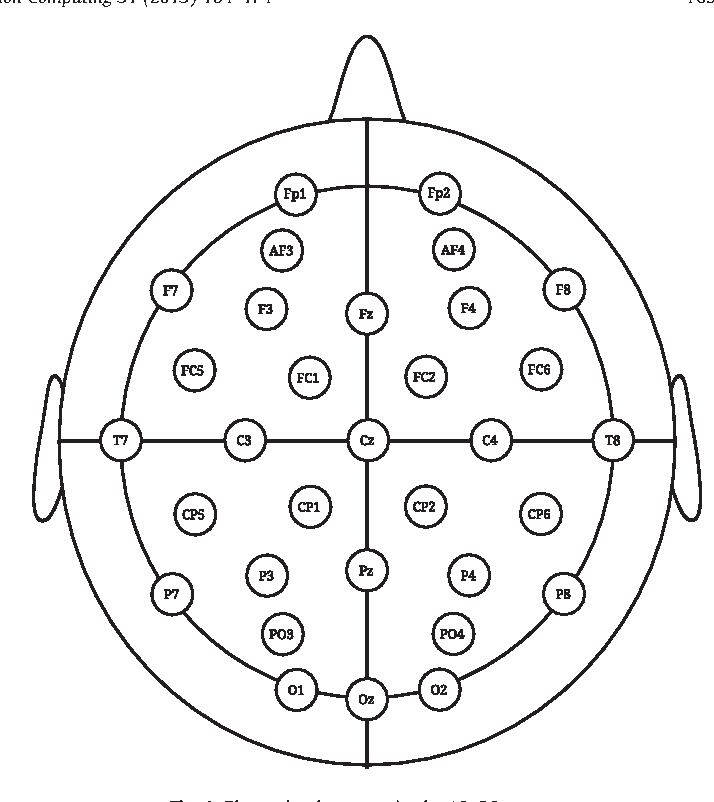
\includegraphics[width=0.4\textwidth]{recursos_img/configuracion_diagrama_10_20.png}  % Ajusta la ruta y el ancho según sea necesario
    \caption{Configuración 10/20 para colocación de electrodos.}
    \label{fig:mi_imagen}  % Etiqueta para referencias cruzadas en el documento
\end{figure}
Para al colocación de electrodos a la hora de llevar acababo la ejecución del 
experimento se deberá de elegir una configuaración específica dentro de  la 
configuración 10/20 por lo que se debrán de colocar 8 electrodos dentro de las 32 
posibles ubicaciones mostradas en la figura anterior.

\section{Aspectos Éticos y de Bioseguridad}
El estudio será realizado siguiendo los principios éticos de investigación, 
incluyendo el consentimiento informado de los participantes y la protección de su 
privacidad. Se tomarán medidas para asegurar que los datos recolectados sean 
confidenciales y se almacenarán de manera segura. Además, se garantizará que el 
uso de los equipos no suponga ningún riesgo para la salud de los participantes.

\section{Documentos complementarios}
Se adjuntarán los siguientes documentos complementarios:
\begin{itemize}
    \item Consentimiento informado.
    \item Protocolos de seguridad.
    \item Formularios de recolección de datos.
    \item Procedimientos de análisis de datos.
\end{itemize}

\end{document}
